% !TeX root = trigonometric-functions.tex

\chapter{The Pedagogy of the Functional Approach}

\section{The definition of the trigonometric functions}

We will show how the functional approach enables an operational definition of the  trigonometric functions on numerical values that represent rotations in units of radians.
A significant advantage of this approach is that it overcomes the ambiguity of using the word ``degrees,'' once as a measure of angles and again as a measure of rotations.
In the functional approach, the trigonometric functions are defined in a manner that is consistent with the abstract concept of function already known to middle-school students. The idiosyncratic definitions based upon geometric constructions (triangles) are not needed. The domain of the functions is the lengths of arcs obtained by rotating a ray from the origin that intersects the circumference of the unit circle centered at the origin (cf. \cite{moore}).

\section{Why radians?}

A function is defined by as a mapping between elements of a domain and elements of a range. The only test that a function must ``pass'' is that an element of a domain can be mapped into at most one element of the range.

There is no reason that the sine function could not be defined on rotation measured in degrees, where one degree is $1/360$ of the rotation around the circumference of the circle. However, it is essential to recognize that the sine function defined on a variable measured in degrees is not the same as the sine function defined on a variable measured in radians. This can be seen in 
Figure~\ref{fig.degrees-or-radians}, which displays graphs of these two functions on the \emph{same} coordinate system!

\begin{figure}[htb]
\begin{center}
\begin{tikzpicture}[scale=1.1]
\draw[step=10mm,white!50!black,thin] (-3,-2) grid (8,2);
\draw (-3,0) -- (8,0);
\draw (0,-2) -- (0,2);
\foreach \x in {-2,-1,1,2,3,4,5,6,7}
  \node at (\x,-.3) {$\x$};
\foreach \y in {-1,-.5,0,.5,1}
  \node at ($(-.3,0)+(0,2*\y)$) {$\y$};
\draw[red,domain=-3:8,samples=100,thick] plot (\x,{2*sin (\x)});
\draw[blue,domain=-3:8,samples=100,thick] plot (\x,{2*sin (\x r)});
\node[blue] at (3.4,1.4) {$\sin x_{\scriptstyle radians}$};
\node[red] at (5,.5) {$\sin x_{\scriptstyle degrees}$};
\end{tikzpicture}
\caption{The sine function when values in the domain are in radians or degrees}\label{fig.degrees-or-radians}
\end{center}
\end{figure}

\newpage

For the value $1.57$, the value of the sine function depends on the unit of measure, and the difference between radians and degrees is quite large:
\[
\sin\: 1.57_{\scriptstyle radians} \approx 1\,,\;\;\;\;\; \sin \: 1.57_{\scriptstyle degrees}\approx 0.027\,.
\]

Apparently, when we teach trigonometric functions on both degrees and radians, students are unaware of the different representations of the graphs. In practice, students seem to regard the domain of trigonometric function as ``rotations,'' and the units of measurement of the domain of rotations are not important. This leads to inconsistent graphs, where the domain on the $x$-axis is labeled with two different units of measure (Figure~\ref{fig.both-radians-and-degrees}).
 
\begin{figure}[hbt]
\begin{center}
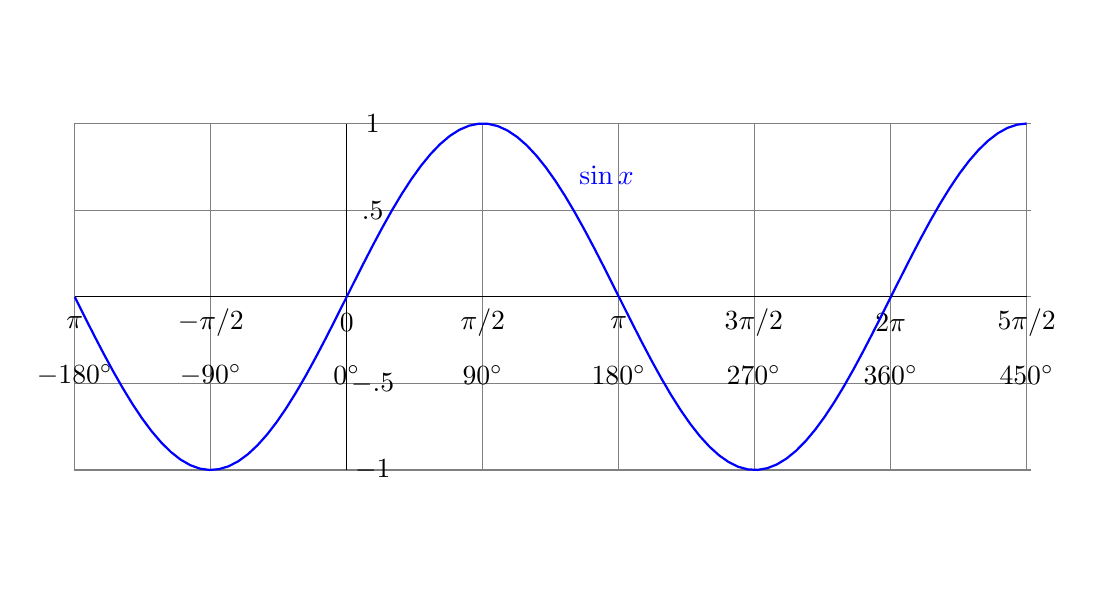
\begin{tikzpicture}[scale=1.1]
\draw[xstep=1.57,ystep=10mm,white!50!black,thin] (-3.15,-2) grid (7.9,2);
\foreach \x/\rad/\deg in {-3.14/\pi/-180^\circ,-1.57/{-\pi/2}/-90^\circ,0/0/0^\circ,1.57/{\pi/2}/90^\circ,3.14/\pi/180^\circ,4.7/{3\pi/2}/270^\circ,6.28/2\pi/360^\circ,7.85/{5\pi/2}/450^\circ} {
  \node at (\x,-.3) {$\rad$};
  \node at (\x,-.9) {$\deg$};
}
\foreach \y/\s in {-3/,-2/-1,-1/-.5,1/.5,2/1,3/} {
  \node at (.3,\y) {$\s$};
}
\draw (-3.14,0) -- (7.85,0);
\draw (0,-2) -- (0,2);
\draw[blue,domain=-3.14:7.85,samples=100,thick] plot (\x,{2*sin (\x r)});
\node[blue] at (3,1.4) {$\sin x$};
\end{tikzpicture}
\caption{Inconsistent units of measures for the same domain}\label{fig.both-radians-and-degrees}
\end{center}
\end{figure}

This dual representation is particularly problematic when discussing the covariance between the values of $x$ and $\sin x$, that is, when studying the derivative of the sine function.
From Figure~\ref{fig.degrees-or-radians} it can seen that \emph{slopes} (and hence the derivatives) of $\sin x_{\scriptstyle \textit{radians}}$ (Figure~\ref{fig.derivative-in-radians}) and $\sin x_{\scriptstyle \textit{degrees}}$ (Figure~\ref{fig.derivative-in-degrees}) are different for equal values of $x$. 

\begin{figure}[htb]
\begin{center}
\begin{tikzpicture}[scale=1.1]
\draw[step=10mm,white!50!black,thin] (-2,-2) grid (7,2);
\draw (-2,0) -- (7,0);
\draw (0,-2) -- (0,2);
\foreach \x in {-2,-1,1,2,3,4,5,6,7}
  \node at (\x,-.3) {$\x$};
\foreach \y in {-1,-.5,0,.5,1}
  \node at ($(-.3,0)+(0,2*\y)$) {$\y$};
\draw[red,domain=-2:7,samples=100,thick] plot (\x,{2*sin (\x r)});
\draw[blue,domain=-2:7,samples=100,thick] plot (\x,{2*cos (\x r)});
\node[red] at (2.2,1.4) {$\sin\: x_{\scriptstyle radians}$};
\node[blue] at (4.4,1.4) {$\sin'\: x_{\scriptstyle radians}$};
\end{tikzpicture}
\caption{The sine function and its derivative in radians}\label{fig.derivative-in-radians}
\end{center}
%\end{figure}

%\begin{figure}[htb]
\begin{center}
\begin{tikzpicture}[scale=1.2]
\draw[step=10mm,white!50!black,thin] (-2,-2) grid (6,2);
\draw (-2,0) -- (6,0);
\draw (0,-2) -- (0,2);
\foreach \x/\deg in {-2/-400,-1/-200,1/200,2/400,3/600,4/800,5/1000,6/1200}
  \node at (\x,-.3) {$\deg$};
\foreach \y in {-1,-.5,0,.5,1}
  \node at ($(-.3,0)+(0,2*\y)$) {$\y$};
\draw[red,domain=-400:1200,samples=100,thick] plot (0.005*\x,{2*sin (\x)});
\draw[blue,domain=-400:1200,samples=100,thick] plot (0.005*\x,{.05*cos (\x)});
\node[red] at (3.2,1.6) {$\sin\: x_{\scriptstyle degrees}$};
\node[blue] at (1,.3) {$\sin'\: x_{\scriptstyle degrees}$};
\end{tikzpicture}
\caption{The sine function and its derivative in degrees}\label{fig.derivative-in-degrees}
\end{center}
\end{figure}

To understand the graph of $\sin'\: x_{\scriptstyle degrees}$ recall that:
\[
\sin' x=\lim_{h\rightarrow 0} \disfrac{\sin(x+h)-\sin(x)}{h}\,.
\]
For $x=90$ and $h=10$:
\[
\disfrac{\sin(x+h)-\sin(x)}{h} = \disfrac{\sin 100^\circ-\sin 90^\circ}{10}\approx \disfrac{-0.0152}{10}=-0.00152\,,
\]
so we see why the value of $\sin'\: x_{\scriptstyle degrees}$ is very small.

We must choose one of the two representations.
From Figures~\ref{fig.derivative-in-radians},~\ref{fig.derivative-in-degrees}, we can see that the derivative of $\sin'\: x_{\scriptstyle radians}$ is $\cos\: x_{\scriptstyle radians}$ while the derivative of $\sin'\: x_{\scriptstyle degrees}$ is $a\cdot\cos x_{\scriptstyle degrees}$ where $a\ll 1$.
We can justify the choice of defining the trigonometric functions on a domain measured in radians for reasons of mere convenience.
Of course, there are other considerations for selecting radians and these will be discussed below.

\section{Periodic functions: the winding operation}

Trigonometric functions are \emph{periodic}.
While it is possible to discuss periodic functions initially in the context of trigonometry, we suggest that the topic be discussed earlier.\footnote{The following activity was shown to us by Zippora Resnick.}

\begin{wrapfigure}[11]{r}{.5\textwidth}
%\begin{figure}[hbt]
\begin{center}
\vspace{-6ex}
\begin{tikzpicture}[scale=1.2]
\draw[step=10mm,white!50!black,thin] (-2,-2) grid (4,2);
\draw (-2,0) -- (4,0);
\draw (0,-2) -- (0,2);
\foreach \x in {-2,-1,0,1,2,3,4}
  \node at (\x,-.3) {$\x$};
\foreach \y in {-2,-1,0,1,2}
  \node at ($(-.5,0)+(0,\y)$) {$\y$};
\coordinate (X) at (3.3,0);
\draw[red,very thick,->] (0,0) -- (3.25,0);
\draw[red,very thick] (1,0) -- (1,1) -- (-1,1);
\coordinate (P) at (-1,.7);
\draw[red,very thick,->] (-1,1) -- (-1,.75);
\draw[thick] (P) -- (-1,-1) -- (1,-1) -- (1,0);
\coordinate (S) at (3.3,0.7);
\draw[blue,very thick,dashed,->] (P) -- (3.2,0.7);
\draw[blue,very thick,dashed,<-] (3.3,.65) -- (3.3,0);
\fill[blue] (S) circle(1.5pt) node[above] {$S=(3.3,0.7)$};
\fill (X) circle(1.5pt) node[below,yshift=-4pt] {$X$};
\fill (1,0) circle(1.5pt) node[above right] {$B$};
\fill[red] (P) circle(1.5pt) node[left] {$P$};
\end{tikzpicture}
\caption{Winding a thread around a square}\label{fig.winding-around-a-square}
\end{center}
%\end{figure}
\end{wrapfigure}

We construct a function that maps real numbers to real numbers, where the domain is the set of lengths obtained by winding a thread (real or imaginary) around a geometric shape, \emph{not necessarily a circle}.
Consider a square centered at the origin of the coordinate system, oriented so that its its sides are parallel to the axes and the length of each side is two units (Figure~\ref{fig.winding-around-a-square}).
For any given value of $x$, take a thread of length $|x|$ and wind it around the square starting $(1,0)$. As usual the thread is wound counterclockwise $x>0$ and clockwise if $x <0$.
Label the point on the square reached at the end of the thread by $P$.


Let us construct the function that maps of the length of the thread $x$ to the $y$ coordinate of $P$. In the Figure, we see that $x=3.3$ is mapped into $y=0.7$.
This function is periodic with a period equal to the perimeter of the square: $f(x+8k)=f(x), k\in \mathcal{Z}$.

A fruitful exercise for students is to explore the winding operation for various polygons (\geoproject{g.winding}).


\begin{itemize}
\item \url{https://www.geogebra.org/m/QRmStjFg} is another project on periodic functions.
\item \url{https://scratch.mit.edu/studios/25046732} is a collection of programs in Scratch that demonstrate winding around a circle.
\end{itemize}


\section{The function \texorpdfstring{$s$}{s} maps a real number to a coordinate}

In the previous section, we defined a function by winding a thread around a polygon. As the number of sides of a (regular) polygon increases, the polygon converges to a circle. The trigonometric functions are defined by winding around a unit circle: a circle of radius $1$ centered at $(0,0)$. The beginning of the thread is at $(1,0)$. The functions will be periodic with period the ``perimeter'' (circumference) of the circle, $2\pi$.

Figure~\ref{fig.winding-around-a-square} shows a correlation between two points, $P$ on the perimeter of the polygon and $S$, the point defined by the intersection of a horizontal line through $P$ and a vertical line through $X$.
However, a function is defined as a mapping between a value in its domain to a value in its range, not as a correlation between two points, each with an $x$ and $y$ value.
Therefore, we define a function $s(x)$ that maps the $x$ value of $S$ and $X$ (only) to the $y$ value of $P$ and $S$.

Of course, teachers immediately see that $s$ is the sine function, but they must consider if they wish to point this out to the students.
In the functional approach, it makes sense to defer discussing the relationship with trigonometric functions defined in right triangles, which the students possibly know from previous study of mathematics and physics.
The reason is that the concept of a function as a mapping from all real numbers to points on the unit circle should be firmly established before making the transition to the triangular definitions.

\begin{figure}[hbt]
\begin{center}
\begin{tikzpicture}[scale=1.5]
\begin{scope}
\draw[step=10mm,white!50!black,thin] (-2,-2) grid (2,2);
\draw (-2,0) -- (2,0);
\draw (0,-2) -- (0,2);
\foreach \x in {-1,-.5,0,.5,1}
  \node at (2*\x,-.2) {$\scriptstyle \x$};
\foreach \y in {-1,-.5,.5,1}
  \node at ($(-.2,0)+(0,2*\y)$) {$\scriptstyle \y$};
\coordinate (O) at (0,0);
\coordinate (B) at (2,0);
\coordinate (P) at (55:2);
\fill (O) circle(1pt) node [below left] {$O$};
\fill (B) circle(1pt);
\fill[red] (P) circle(1pt) node [above right] {$P$};
\node[draw, name path = circle] at (O)
    [circle through = (P)] {};
\draw[red,thick] (B) arc[start angle=0,end angle=55,radius=2cm];
\node[red] at (1.6,1.5) {$\textsf{arc}$};
\draw[blue,thick] (P) -- (P |- O);
\end{scope}
\begin{scope}[xshift=5cm]
\draw[xstep=1.57,ystep=10mm,white!50!black,thin] (-1.57,-2) grid (3.14,2);
\draw (-1.57,0) -- (3.14,0);
\draw (0,-2) -- (0,2);
\foreach \x/\tick in {-1.57/{-\pi/4},1.57/{\pi/4},3.14/{\pi/2}}
  \node at (\x,-.2) {$\tick$};
\foreach \y in {-1,-.5,0,.5,1}
  \node at ($(-.2,0)+(0,2*\y)$) {$\scriptstyle \y$};
\coordinate (O) at (0,0);
\coordinate (B) at (2,0);
\fill (O) circle(1pt) node [above right] {$O$};
\coordinate (S) at (1*2,.819*2);
\fill[teal] (S) circle(1pt)
  node [above left,xshift=8pt] {\textsf(arc,\ y value of P)}
  node[right,teal] {$\bm{S}$};
\draw [thick,teal] (S) -- (S |- O) coordinate (X);
\draw[thick,red] (O) -- node[below] {\textsf{arc}} (X);
\fill[teal] (X) circle(1pt) node[above right] {$\bm{X}$};
\end{scope}
\end{tikzpicture}
%\includegraphics[width=\textwidth,keepaspectratio]{sine-radians-split}
\caption{Definition of the function $s(x)$}\label{fig.function-s}
\end{center}
\end{figure}

Figure~\ref{fig.function-s} (\geoproject{g.sine}) shows the definition of the function $s(x)$ in a split window: the right window shows the independent variable (point $X$) and the dependent variable (point $S$), which is the value of the function . The left window shows the geometric construction that defines the function.\footnote{In Geogebra, constructions such as these can be done in a single screen (\geoproject{g.single}) or in a split screen (\geoproject{g.split}).}
The $x$-value of $X$, the independent variable, is used as the length of an arc from point $(1,0)$ around the circumference of the unit circle.
The $y$-value of $P$, the dependent variable, is the length of a perpendicular line from $P$ to the $x$-axis.


%\begin{figure}[hbt]
\begin{wrapfigure}[8]{r}{.6\textwidth}
\begin{center}
\vspace{-5ex}
\begin{tikzpicture}[scale=.95]
\draw[xstep=1.57cm,ystep=1cm,white!50!black,thin]
  (-1.58,-2) grid (7.86,2);
\draw (-1.57,0) -- (7.85,0);
\draw (0,-2) -- (0,2);
\foreach \x/\tick in {-1.57/{-\pi/2},0/0,1.57/{\pi/2},3.14/{\pi},4.71/{3\pi/2},6.28/{2\pi},7.85/{5\pi/4}}
  \node at (\x,-.3) {$\scriptstyle \tick$};
\foreach \y in {-1,-.5,.5,1}
  \node at ($(-.3,0)+(0,2*\y)$) {$\scriptstyle \y$};
\path[red,domain=-1.5:7.85,samples=40,mark=*,mark size=1pt] plot (\x,{2*sin (\x r)});
\coordinate (P) at (.960,.819*2);
\coordinate (O) at (0,0);
\fill (O) circle(2pt) node [below left] {$O$};
\fill[red] (P) circle(2pt) node [above,yshift=8pt] {\textsf(arc,y value of P)};
\draw [very thick,teal] (P) -- (P |- O) coordinate (X);
\fill[teal] (X) circle(2pt) node[above right] {$X$};
\end{tikzpicture}
%\includegraphics[width=\textwidth,keepaspectratio]{trace-of-the-function}
\caption{Trace of the function $s$}\label{fig.trace-of-the-function}
\end{center}
%\end{figure}
\end{wrapfigure}

The graphical representation of the function for all real values can be obtained by tracing the points $P$ as you drag the point $X$ left and right (Figure~\ref{fig.trace-of-the-function}, \geoproject{g.trace})

The graphical representation reveals the periodicity of the function: $s(x) = s(x + 2\pi k), k\in \mathcal{Z}$.

\section{Symmetries of the function \texorpdfstring{$s$}{s}}

When winding around a circle (as when winding around a square), by symmetry there are close relationships between values of the functions for points $P$ located in the four quadrants.
Clearly, for every point $P_1$ in the first quadrant there is a point $P_2$ in the second quadrant with $x_2=-x_1$ and $y_2=y_1$.
These relationships can be explored by the students even before the trigonometric functions are defined.

Figure~\ref{fig.symmetries} (left) displays points obtained by reflections of the point $P$ which is the endpoint of the arc starting from $(1,0)$. The following table lists the points obtained by reflection:
\begin{center}
\begin{tabular}{|l|l|}
\hline
$P$ & Endpoint of the arc\\\hline
$P_x$ & Reflection around the $x$-axis\\\hline
$P_y$ & Reflection around the $y$-axis\\\hline
$P_{xy}$ & Reflection around the origin\\\hline
\end{tabular}
\end{center}

\bigskip

\begin{figure}[hbt]
\begin{minipage}{.45\textwidth}
\begin{center}
\begin{tikzpicture}[scale=1.2]
\draw[step=10mm,white!50!black,thin] (-3,-3) grid (3,3);
\draw[thin] (-3,0) -- (3,0);
\draw[thin] (0,-3) -- (0,3);
  \coordinate[label = above left:$A$]  (A) at (-2,0);
  \coordinate[label = above right:$B$] (B) at (2,0);
  \coordinate[label = above left:$O$] (O) at (0,0);
%  \coordinate[label = above right:$H$] (H) at (0,2);
%  \coordinate[label = below right:$G$] (G) at (0,-2);
  \fill (A) circle (1.5pt);
  \fill (B) circle (1.5pt);
  \fill (O) circle (1.5pt);
%  \fill (H) circle (1.5pt);
%  \fill (G) circle (1.5pt);
  \coordinate (P) at (65:2);
  \coordinate (Py) at (115:2);
  \coordinate (Pxy) at (-115:2);
  \coordinate (Px) at (-65:2);
  \fill[red] (P) circle (1.5pt) node[above right] {$P$};
  \fill[red] (Pxy) circle (1.5pt) node[below left] {$P_{xy}$};
  \fill[red] (Py) circle (1.5pt) node[above left] {$P_y$};
  \fill[red] (Px) circle (1.5pt) node[below right] {$P_x$};
\foreach \x/\tick in {-2/-1,-1/-.5,0/0,1/.5,2/1}
  \node[below left] at (\x,0) {$\scriptstyle\tick$};
\foreach \y/\tick in {-2/-1,-1/-.5,1/.5,2/1}
  \node[below left] at (0,\y) {$\scriptstyle\tick$};
  \node[draw, name path = circle] at (O)
    [circle through = (A)] {};
\draw[red,very thick] (B) arc[start angle=0,end angle=65,radius=2cm];
\node[red] at (1.8,1.4) {\textsf{arc}};
\end{tikzpicture}
\end{center}
\end{minipage}
\hspace{2em}
\begin{minipage}{.45\textwidth}
\begin{center}
\begin{tikzpicture}[scale=1.2]
\draw[step=10mm,white!50!black,thin] (-3,-3) grid (3,3);
\draw[thin] (-3,0) -- (3,0);
\draw[thin] (0,-3) -- (0,3);
  \coordinate[label = above left:$A$]  (A) at (-2,0);
  \coordinate[label = above right:$B$] (B) at (2,0);
  \coordinate[label = above left:$O$] (O) at (0,0);
%  \coordinate[label = above right:$H$] (H) at (0,2);
%  \coordinate[label = above right:$G$] (G) at (0,-2);
  \fill (A) circle (1.5pt);
  \fill (B) circle (1.5pt);
  \fill (O) circle (1.5pt);
%  \fill (H) circle (1.5pt);
%  \fill (G) circle (1.5pt);
  \coordinate (P) at (30:2);
  \coordinate (Py) at (150:2);
  \coordinate (Pxy) at (-150:2);
  \coordinate (Px) at (-30:2);
  \fill[red] (P) circle (1.5pt) node[above right] {$P$};
  \fill[red] (Pxy) circle (1.5pt) node[below left] {$P_{xy}$};
  \fill[red] (Py) circle (1.5pt) node[above left] {$P_y$};
  \fill[red] (Px) circle (1.5pt) node[below right] {$P_x$};
\foreach \x/\tick in {-2/-1,-1/-.5,0/0,1/.5,2/1}
  \node[below left] at (\x,0) {$\scriptstyle\tick$};
\foreach \y/\tick in {-2/-1,-1/-.5,1/.5,2/1}
  \node[below left] at (0,\y) {$\scriptstyle\tick$};
  \node[draw, name path = circle] at (O)
    [circle through = (A)] {};
\draw[red,very thick] (B) arc[start angle=0,end angle=30,radius=2cm];
\draw[red,very thick] (A) arc[start angle=180,end angle=150,radius=2cm];
\draw[blue,very thick] (P) arc[start angle=30,end angle=150,radius=2cm];
\node[red] at (2.2,.8) {\textsf{arc}};
\end{tikzpicture}
\end{center}
\end{minipage}
\caption{Symmetries of the function $s$}\label{fig.symmetries}
\end{figure}


By examining the Figure we conclude that:
\begin{eqnarray*}
s(P_x) &=& -s(P)\\
s(P_y) &=& s(P)\\
s(P_{xy}) &=& -s(P)\,.
\end{eqnarray*}

Consider now Figure~\ref{fig.symmetries} (right). Since $P_y$ is the reflection of $P$ about the $y$ axis, the length of the arc from $A$ to $P_y$ is the same as the length of the arc from $B$ to $P$. Therefore, if the length of the arc from $A$ to $P_y$ is $x$, the length of the arc from $B$ to $P_y$ is $\pi-x$, so we conclude that:
\[
s(x) = s(\pi - x)\,.
\]
Since $P$ was chosen arbitrarily, this is true for any $x$.

Additional symmetries can be derived in the same way:
\begin{eqnarray*}
s(x) &=& -s(-x)\\
s(\pi+x) &=& -s(x)\\
s(\pi-x) &=& s(x)\,.
\end{eqnarray*}
From $s(x) = -s(-x)$ it follows that the function is odd.

The cyclic and symmetrical properties facilitate obtaining values of the function $s$. This of great help to students since they need remember only a few values of $s$.

\newpage

%\begin{figure}[hbt]
\begin{wrapfigure}[12]{r}{.6\textwidth}
\begin{center}
\vspace{-2ex}
\begin{tikzpicture}[scale=1.3]
  \draw[step=10mm,white!50!black,thin] (-3,-3) grid (3,3);
  \draw[thin] (-3,0) -- (3,0);
  \draw[thin] (0,-3) -- (0,3);
  \coordinate[label = above right:$B$] (B) at (2,0);
  \coordinate[label = above left:$O$] (O) at (0,0);
  \fill (B) circle (1.5pt);
  \fill (O) circle (1.5pt);
  \coordinate (P) at (30:2);
  \coordinate (Py) at (150:2);
  \coordinate (Pxy) at (-150:2);
  \coordinate (Px) at (-30:2);
  \fill[red] (P) circle (1.5pt) node[black,above right]
     {
      \shortstack{
         $\left(\disfrac{\pi}{6}\;,
             \disfrac{1}{2}\right)$
      \\
      $\left(-\bm{?},
             \disfrac{1}{2}\right)$}};
  \fill[red] (Pxy) circle (1.5pt) node[below left,black]
     {
      \shortstack{
         $\left(\;\;\;\bm{?},
             -\disfrac{1}{2}\right)$
      \\
      $\left(-\bm{?},
             -\disfrac{1}{2}\right)$}};
  \fill[red] (Py) circle (1.5pt) node[above left,black]
     {
      \shortstack{
         $\left(\;\;\;\bm{?},
             \disfrac{1}{2}\right)$
      \\
      $\left(-\bm{?},
             \disfrac{1}{2}\right)$}};
  \fill[red] (Px) circle (1.5pt) node[below right,black]
     {
      \shortstack{
         $\left(\;\;\;\bm{?},
             -\disfrac{1}{2}\right)$
      \\
      $\left(-\bm{?},
             -\disfrac{1}{2}\right)$}};
  \node[draw, name path = circle] at (O)
    [circle through = (B)] {};
  \draw[red,very thick] (B)
     arc[start angle=0,end angle=30,radius=2cm];
\end{tikzpicture}
\caption{Computing values of the function $s$}\label{fig.computing}
\end{center}
%\end{figure}
\end{wrapfigure}

A good exercise at this point is to identify the values $V=\{x_1,x_2,\ldots\}$ of $x$ that such that $s(x_i)=\pm s(x)$. Suppose we know that $s(\pi/6)=1/2$. We now ask for the value of $x$ for the three symmetrical points (Figure~\ref{fig.computing}). Each point is also reached by winding the thread around the circle in a negative direction. Finally, since the function is periodic, for example, $s(-5\pi/6)=1/2$, $V=\{x_1,x_2,\ldots\}$ is an infinite set.

\vspace{10ex}

\section{The function \texorpdfstring{$c$}{c} maps a real number to a coordinate}

The definition of the function $s$ leads naturally to the definition of a function $c$ which maps a real number (the length of an arc on the circumference of the unit circle) to the $x$-value of the end point of the arc (Figure~\ref{fig.cosine}, \geoproject{g.cosine}).
\begin{figure}[H]
\begin{center}
\begin{tikzpicture}[scale=1.6]
\begin{scope}
\draw[step=10mm,white!50!black,thin] (-2,-2) grid (2,2);
\draw (-2,0) -- (2,0);
\draw (0,-2) -- (0,2);
\foreach \x in {-1,-.5,.5,1}
  \node at (2*\x,-.2) {$\scriptstyle \x$};
\foreach \y in {-1,-.5,0,.5,1}
  \node at ($(-.2,0)+(0,2*\y)$) {$\scriptstyle \y$};
\coordinate (O) at (0,0);
\coordinate (B) at (2,0);
\coordinate (P) at (55:2);
\fill (O) circle(1pt) node [below left] {$O$};
\fill (B) circle(1pt);
\fill[red] (P) circle(1pt) node [above right] {$P$};
\node[draw, name path = circle] at (O)
    [circle through = (P)] {};
\draw[red,thick] (B) arc[start angle=0,end angle=55,radius=2cm];
\node[red] at (1.6,1.5) {$\textsf{arc}$};
\draw[blue,thick] (P) -- (P -| O);
\end{scope}
\begin{scope}[xshift=4.5cm]
\draw[xstep=1.57,ystep=10mm,white!50!black,thin] (-1.57,-2) grid (3.14,2);
\draw (-1.57,0) -- (3.14,0);
\draw (0,-2) -- (0,2);
\foreach \x/\tick in {-1.57/{-\pi/4},1.57/{\pi/4},3.14/{\pi/2}}
  \node at (\x,-.2) {$\tick$};
\foreach \y in {-1,-.5,0,.5,1}
  \node at ($(-.2,0)+(0,2*\y)$) {$\scriptstyle \y$};
\coordinate (O) at (0,0);
\coordinate (B) at (2,0);
%\coordinate (P) at (.960*2,.574*2);
\coordinate (S) at (1*2,.574*2);
\fill (O) circle(1pt) node [below left] {$O$};
\fill (B) circle(1pt);
\fill[teal] (S) circle(1pt) node [teal,above left,xshift=8pt]
   {\textsf(arc,\ x value of P)}
   node[right,teal] {$\bm{S}$};
\draw [thick,teal] (S) -- (S |- O) coordinate (X);
\draw[thick,red] (O) -- node[below] {\textsf{arc}} (X);
\fill[teal] (X) circle(1pt) node[above right] {$\bm{X}$};
\end{scope}
\end{tikzpicture}
%\includegraphics[width=\textwidth,keepaspectratio]{sine-radians-split}
\caption{Geometric construction that defines the function $c(x)$}\label{fig.cosine}
\end{center}
\end{figure}

Be careful: the notation may lead to confusion.
The \emph{point} $X$ (upper case) identifies a point along the $x$-axis. The length from the origin to $X$ specifies the length of the arc from $(1,0)$ around the circumference of the circle.
The \emph{variable} $x$ (lower case) is the $x$ value of the coordinates of $P$, the endpoint of this arc.

In the Geogebra project, a trace of the value of $c(x)$ as $x$ is moved along the $x$-axis gives a graphical representation of the function (Figure~\ref{fig.cosine-trace}).

\begin{figure}[hbt]
\begin{center}
\begin{tikzpicture}[scale=1.6]
\begin{scope}
\draw[step=10mm,white!50!black,thin] (-2,-2) grid (2,2);
\draw (-2,0) -- (2,0);
\draw (0,-2) -- (0,2);
\foreach \x in {-1,-.5,.5,1}
  \node at (2*\x,-.2) {$\scriptstyle \x$};
\foreach \y in {-1,-.5,0,.5,1}
  \node at ($(-.2,0)+(0,2*\y)$) {$\scriptstyle \y$};
\coordinate (O) at (0,0);
\coordinate (B) at (2,0);
\coordinate (P) at (130:2);
\fill (O) circle(1pt) node [below left] {$O$};
\fill (B) circle(1pt);
\fill[red] (P) circle(1pt) node [above left] {$P$};
\node[draw, name path = circle] at (O)
    [circle through = (P)] {};
\draw[red,thick] (B) arc[start angle=0,end angle=130,radius=2cm];
\node[red] at (1.6,1.5) {$\textsf{arc}$};
\draw[blue,thick] (P) -- (P -| O);
\end{scope}
\begin{scope}[xshift=4.5cm]
\draw[xstep=1.57cm,ystep=1cm,white!50!black,thin] (-1.58,-2) grid (3.16,2);
\draw (-1.57,0) -- (3.16,0);
\draw (0,-2) -- (0,2);
\foreach \x/\tick in {-1.57/{-\pi/2},1.57/{\pi/2},3.14/{\pi}}
  \node at (\x,-.3) {$\tick$};
\foreach \y in {-1,-.5,0,.5,1}
  \node at ($(-.3,0)+(0,2*\y)$) {$\scriptstyle\y$};
\draw[thick,teal,domain=-1.56:3.15,samples=100] plot (\x,{2*cos (\x r)});
\coordinate (S) at (2.269,-.64*2);
\coordinate (O) at (0,0);
\fill (O) circle(1pt) node [below left] {$O$};
\fill[teal] (S) circle(1pt) node [right] {$S$}
  node[left,xshift=-4pt] {\textsf(arc,x value of P)};
\draw [very thick,teal] (S) -- (S |- O) coordinate (X);
\draw[very thick,red] (O) -- node[above] {\textsf{arc}} (X);
\fill[teal] (X) circle(1pt) node[above right] {$X$};
\end{scope}
\end{tikzpicture}
%\includegraphics[width=\textwidth,keepaspectratio]{sine-radians-split}
\caption{Trace of the function $c(x)$}\label{fig.cosine-trace}
\end{center}
\end{figure}

From Figures~\ref{fig.symmetries}, symmetry properties of $c(x)$ can be derived. We leave it to the reader to justify the following equalities:
\begin{eqnarray*}
c(P_x) &=& c(P)\\
c(P_y) &=& -c(P)\\
c(P_{xy}) &=& -c(P)\,.
\\
c(x) &=& -c(\pi - x)\\
c(x) &=& c(-x)\\
c(\pi+x) &=& -c(x)\\
c(\pi-x) &=& -c(x)\,.
\end{eqnarray*}
Figure~\ref{fig.computing} can be modified to ask questions about the function $c(x)$.

At this point, the teacher faces the dilemma whether to continue the study of the sine and cosine functions (specifically, translation and change of radius) or the move on the tangential trigonometric functions.
Both choices are legitimate.
There is a significant advantage to continuing with the trigonometric functions already presented. 
This can firmly establish the concept that trigonometric functions are true functions that can be modified by performing arithmetic operations of the domain values or on the range values.
Once this has been done, the tangential functions can be taught.

Translation and change of radius is discussed in a separate Chapter~\ref{ch.translated}.



\section{Tangential trigonometric functions}

The standard approach is to define the tangent function as a correlation between a real number (that defines the length and direction of an arc) and the $y$ value of the intersection of (1) the line passing through the center of the coordinate system and the endpoint of the arc $P$, and (2) a vertical line tangent to the unit circle at $(1,0)$ (Figure~\ref{fig.tangent}, \geoproject{g.tangent}).

\begin{figure}[hbt]
\begin{center}
\begin{tikzpicture}
\begin{scope}[scale=.6]
\draw[step=2cm,white!50!black,thin] (-6.05,-6.05) grid (6,6);
\draw[thin] (-6,0) -- (6,0);
\draw[thin] (0,-6) -- (0,6);
  \coordinate (A) at (-4,0);
  \coordinate[label = above right:$B$] (B) at (4,0);
  \coordinate[label = above left:$O$] (O) at (0,0);
  \draw (O) -- (6,0);
  \node[draw, thick, name path = circle] at (O)
    [circle through = (A)] {};
  \coordinate (TT) at (53:7.5);
  \draw[dashed,name path=side,->] ($(O)!-1.05!(TT)$) -- (TT);
  \draw[name path=tangent,dashed] (4,-6) -- (4,6);
  \path [name intersections = {of = circle and side, by = {C}}];
  \path [name intersections = {of = side and tangent, by = {T}}];
  \draw[thick,purple] (B) -- node[right] {$\tan\alpha$} (T);
  \draw[rotate=90] (B) rectangle +(12pt,12pt);
  \draw[thick,red] (B) arc [start angle = 0, end angle = 53, radius=4];
  \node[red] at (3.4,3) {\textsf{arc}};
  \fill[red] (C) circle (3pt) node[above] {$P$};
  \fill[purple] (T) circle (3pt) node[above left,yshift=-2pt] {$T$};
  \fill (O) circle (3pt) node[above right,xshift=10pt] {$\alpha$};
  \fill[purple] (B) circle (3pt);
\end{scope}
\begin{scope}[xshift=6.8cm,scale=1.6]
\draw[xstep=1.57,ystep=1,white!50!black,thin] (-1.57,-2) grid (3.14,2);
\draw (-1.57,0) -- (3.14,0);
\draw (0,-2) -- (0,2);
\foreach \x/\tick in {-1.57/{-\pi/4},0,1.57/{\pi/4},3.14/{\pi/2}}
  \node at (\x,-.2) {$\tick$};
\foreach \y/\tick in {-1/-2,-.5/-1,.5/1,1/2}
  \node at ($(-.2,0)+(0,2*\y)$) {$\scriptstyle \tick$};
\coordinate (O) at (0,0);
\coordinate (Tan) at (.925*2,1.38);
\fill[red] (O) circle(1pt) node [above left,black] {$O$};
\fill[purple] (Tan) circle(1pt) node [above right] {$T$} node[left,xshift=-12pt] {\textsf{(arc, y value of T)}};
\draw[thick,purple] (Tan) -- (Tan |- O) coordinate (X);
\fill[purple] (X) circle(1pt) node[above right] {$X$};
\draw[very thick,red] (O) -- node[below] {\textsf{arc}} (X);
\end{scope}
\end{tikzpicture}
%\includegraphics[width=\textwidth,keepaspectratio]{tangent}
\caption{The tangent function}\label{fig.tangent}
\end{center}
\end{figure}

This definition is consistent with the triangular definition. In the triangle $\triangle TBO$, $\tan \alpha$ is opposite $TB$ over adjacent $OB$ which is $1$ in the unit circle.

The tangent function demonstrates a periodic function with period $\pi$, but it is undefined for an infinite number of real values. This can be seen geometrically: as $\alpha$ approaches $\disfrac{\pi}{2}+\pi k, k in \mathcal{Z}$, the line $OP$ approaches a line parallel to the line $x=1$. The $y$-coordinate of the intersection $T$ becomes larger and larger, approaching infinity.

Conversely, for an arc whose length is any real number $a$, find the point $T=(1,a)$. $TB$ is the tangent of the angle of the line through the intersection of $O$ and $T$ relative to the $x$-axis.
This demonstrates that the tangent function tangent can take any real value.

Similarly, the cotangent function is defined as the intersection of the line through $O$ and $P$ with the horizontal line $y = 1$ (Figure~\ref{fig.cotangent}, \geoproject{g.cotangent}).

This definition is consistent with the triangular definition. In the congruent triangles $\triangle CDO,\triangle C'EO$, $\cot \alpha$ is adjacent $CD$ over opposite $OD$ which is $1$ in the unit circle. Since both the sine and cosine of $\angle BOP$ are the negatives of those of $\angle BOC$, their quotient is positive.


\begin{figure}[hbt]
\begin{center}
\begin{tikzpicture}
\begin{scope}[scale=.6]
\draw[step=2cm,white!50!black,thin] (-6.1,-6) grid (6,6);
\draw[thin] (-6,0) -- (6,0);
\draw[thin] (0,-6) -- (0,6);
  \coordinate[label = above left:$A$] (A) at (-4,0);
  \coordinate[label = above right:$B$] (B) at (4,0);
  \coordinate[label = above left:$D$] (D) at (0,4);
  \coordinate[label = below right:$E$] (E) at (0,-4);
  \coordinate[label = above left:$O$] (O) at (0,0);
  \draw (O) -- (6,0);
  \node[draw, thick, name path = circle] at (O)
    [circle through = (A)] {};
  \coordinate (TT) at (-130:7.5);
  \draw[dashed,name path=side,->] ($(O)!-1.05!(TT)$) -- (TT);
  \draw[name path=cotangent,dashed] (-6,4) -- (6,4);
  \draw[name path=cotangent-prime,dashed] (-6,-4) -- (6,-4);
  \path [name intersections = {of = side and cotangent, by = {C}}];
  \path [name intersections = {of = side and cotangent-prime, by = {Cprime}}];
  \draw[thick,orange] (D) -- node[above] {$\cot\alpha$} (C);
  \draw[thick,orange] (E) -- node[below] {$\cot\alpha$} (Cprime);
  \draw[very thick,teal] (B) arc [start angle = 0, end angle = -130, radius=4];
  \node[teal] at (3.4,-3) {\textsf{arc}};
  \draw[rotate=-90] (D) rectangle +(12pt,12pt);
  \draw[rotate=90] (E) rectangle +(12pt,12pt);
  \fill[orange] (C) circle (3pt) node[above right,xshift=6pt] {$C$} 
     node[below left,black,xshift=-4pt] {$\alpha$};
  \fill[teal] (-130:4) circle (3pt) node[above] {$P$}; 
  \fill (O) circle (3pt);
  \fill[teal] (B) circle (3pt);
  \fill[orange] (D) circle (3pt);
  \fill[orange] (Cprime) circle (3pt) node[below right] {$C'$} 
    node[above right,xshift=6pt,black] {$\alpha$};
  \fill[orange] (E) circle (3pt);
\end{scope}
\begin{scope}[xshift=6cm,scale=1.2]
\draw[xstep=1.57,ystep=1,white!50!black,thin] (-1.57,-3) grid (4.71,3);
\draw (-1.57,0) -- (4.71,0);
\draw (1.57,-3) -- (1.57,3);
\foreach \x/\tick in {-1.57/{-\pi},0/{-\pi/2},1.57/0,3.14/{\pi/2},4.71/{\pi}}
  \node at (\x,-.2) {$\tick$};
\foreach \y in {-1.5,-1,-.5,.5,1,1.5}
  \node at ($(-.2,0)+(1.57,2*\y)$) {$\scriptstyle \y$};
\coordinate (O) at (1.57,0);
\fill (O) circle(1pt) node [above left] {$O$};
\coordinate (X) at (-2.27/2,0);
\fill[teal] (X) circle(1.5pt) node[above left] {$X$};
\coordinate (CT) at (-2.27/2,.839);
\fill[orange] (CT) circle(1.5pt) node[above right] {$\cot\alpha$};
\draw[very thick,teal] (O) -- node[above] {\textsf{arc}} (X);
\draw[very thick,orange] (CT) -- (X);
\draw[orange,domain=-3:-.15,samples=40,thick] plot (\x+1.57,{cot (\x r)/2.5});
\draw[orange,domain=.15:3,samples=40,thick] plot (\x+1.57,{cot (\x r)/2.5});
\end{scope}
\end{tikzpicture}
%\includegraphics[width=\textwidth,keepaspectratio]{cotangent}
\caption{The cotangent function}\label{fig.cotangent}
\end{center}
\end{figure}

Alternatively, the geometric definition can be omitted and cotangent defined by:
\[
\cot x = \frac{1}{\tan x} = \frac{\cos x}{\sin x}\,.
\]

If the geometric definition is used, it would also be necessary to discuss other geometric definitions such as $\tan x = \rule[-12pt]{0pt}{30pt}\disfrac{\sin x}{\cos x}$ and $\sin^2 x+\cos^2 x =1$.
Of course, this involves introducing the triangular approach at this point. 
Furthermore, it will be necessary to take the signs into account (Figure~\ref{fig.signs}, \geoproject{g.signs}).

\begin{figure}[H]
\begin{center}
\begin{tikzpicture}[scale=.63]
\begin{scope}
\draw[step=2cm,white!50!black,thin] (-6.05,-6.05) grid (6,6);
\draw[thin] (-6,0) -- (6,0);
\draw[thin] (0,-6) -- (0,6);
  \coordinate (A) at (-4,0);
  \coordinate (B) at (4,0);
  \coordinate[label = below right:$O$] (O) at (0,0);
  \fill (B) circle (1.5pt);
  \fill (O) circle (1.5pt);
  \node[draw, name path = circle] at (O)
    [circle through = (A)] {};
  \coordinate (point) at (-126:7.4);
  \draw[thick,dashed,name path=side] ($(point)!1.95!(O)$) -- (point);
  \draw[dashed,thick,name path=tangent] (4,-6) -- (4,6);
  \path [name intersections = {of = circle and side, by = {dummy,P}}];
  \fill[red] (P) circle (1pt) node[left,xshift=-4pt] {$P$};
  \draw[thick,blue] (P) -- node[left,xshift=2pt,yshift=6pt] {$\sin x$}
    (P |- O) coordinate (Ps);
  \draw[very thick,teal] (O) -- node[above] {$\cos x$} (Ps);
  \draw[rotate=-90] (Ps) rectangle +(12pt,12pt);
  \draw[rotate=90] (B) rectangle +(12pt,12pt);
  \path [name intersections = {of = side and tangent, by = {T}}];
  \fill (T) circle (1.5pt) node[right]     {$T$};
  \draw[thick,violet] (B) -- node[right] {$\tan x$} (T);
  \draw[thick,red] (B) arc[start angle=0, end angle=-126, radius=4cm];
  \node[red] at (2.6,-3.6) {\textsf{arc}};
\end{scope}
\begin{scope}[xshift=13cm]
\draw[step=2cm,white!50!black,thin] (-6.05,-6.05) grid (6,6);
\draw[thin] (-6,0) -- (6,0);
\draw[thin] (0,-6) -- (0,6);
  \coordinate (A) at (-4,0);
  \coordinate (B) at (4,0);
  \coordinate[label = above left:$O$] (O) at (0,0);
  \fill (B) circle (1.5pt);
  \fill (O) circle (1.5pt);
  \node[draw, name path = circle] at (O)
    [circle through = (A)] {};
\coordinate (point) at (54:7.5);
  \draw[thick,dashed,name path=side] ($(O)!-.98!(point)$) -- (point);
  \draw[dashed,thick,name path=tangent] (4,-6) -- (4,6);
  \path [name intersections = {of = circle and side, by = {P}}];
  \fill[red] (P) circle (1pt) node[above] {$P$};
  \draw[thick,blue] (P) -- node[right,xshift=-1pt,yshift=-8pt] {$\sin x$}
    (P |- O) coordinate (Ps);
  \draw[very thick,teal] (O) -- node[below] {$\cos x$} (Ps);
  \draw[rotate=90] (Ps) rectangle +(12pt,12pt);
  \path [name intersections = {of = side and tangent, by = {T}}];
  \fill (T) circle (1.5pt) node[right]     {$T$};
  \draw[thick,violet] (B) -- node[right] {$\tan x$} (T);
  \draw[thick,red] (B) arc[start angle=0, end angle=54, radius=4cm];
  \node[red] at (3.3,3) {\textsf{arc}};
\end{scope}
\end{tikzpicture}
\caption{Signs of the trigonometric functions}\label{fig.signs}
\end{center}
\end{figure}
